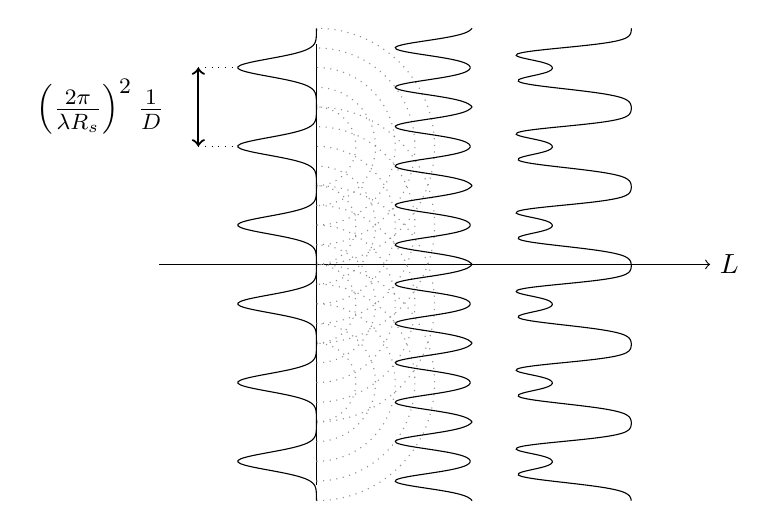
\begin{tikzpicture}
    % Réseau vertical
    \draw[very thin] (0,-2.8) -- (0,2.8);
    
    \draw[->] (-2,0) -- (5,0) node[right]{$L$};
    \foreach \y in {-1.5,-0.5,0.5,1.5} {
    %\draw[->,dashed, lightgray] (0,\y) -- (4,\y+2);
    \draw[dotted, lightgray!25!gray] (0,\y-0.5) arc (-90:90:0.5);
    \draw[dotted, lightgray!25!gray] (0,\y-0.75) arc (-90:90:0.75);
    \draw[dotted, lightgray!25!gray] (0,\y-1) arc (-90:90:1);
    \draw[dotted, lightgray!25!gray] (0,\y-1.25) arc (-90:90:1.25);
    \draw[dotted, lightgray!25!gray] (0,\y-1.5) arc (-90:90:1.5);
    }
    \foreach \y in {-2.5,-1.5,-0.5,0.5,1.5,2.5} {
    \begin{scope}[shift={(0,\y)}]
        \draw[domain=-0.5:0.5,smooth,variable=\x,samples=50, rotate = 90]
        plot ({\x}, {1*exp(-40*\x*\x)});
    \end{scope}
    }

    \foreach \y in {-2.5,-1.5,-0.5,0.5,1.5,2.5} {
    \begin{scope}[shift={(2,\y)}]
        \draw[domain=-0.5:0.5,smooth,variable=\x,samples=50, rotate = 90]
        plot ({\x}, {exp(-60*(\x-0.25)*(\x-0.25))+exp(-60*(\x+0.25)*(\x+0.25))});
    \end{scope}
    }


    \foreach \y in {-2.5,-1.5,-0.5,0.5,1.5,2.5} {
    \begin{scope}[shift={(4,\y)}]
        \draw[domain=-0.5:0.5,smooth,variable=\x,samples=50, rotate = 90]
        plot ({\x}, {
        exp(-85*(\x-0.15)*(\x-0.15))+exp(-85*(\x+0.12)*(\x+0.19))+
        0.5*exp(-85*(\x-0.23)*(\x-0.20))+0.5*exp(-85*(\x+0.25)*(\x+0.25))+
        0.7*exp(-85*\x*\x)});
    \end{scope}
    }

    %\draw[fill = white, color = white] (0,-3) --++ (4,-0.5) -- (0,-4) -- cycle;

    \draw[<->,thick] (-1.5,1.5) -- ++(0,1) node[midway, left = 3mm] {\large $\left(\frac{2\pi}{\lambda R_s}\right)^2\frac{1}{D}$};
    \draw[dotted] (-1.5,1.5) -- ++(0.5,0);
    \draw[dotted] (-1.5,2.5) -- ++(0.5,0);
    
    
\end{tikzpicture}
